\chapter{Diagonalizability}
\label{chapter:23Diag}
 


In the previous chapter, we defined the eigenvalues and eigenvectors of a square matrix $A$.  To each eigenvalue we associate its \emph{algebraic multiplicity}, which is its multiplicity as a root of the characteristic polynomial $\det(A-\lambda I)$ of $A$.  We also associate to each eigenvalue its \emph{geometric multiplicity}, which is the dimension of the associated eigenspace $E_\lambda$.  The key result (Theorem~\ref{thm:limitsmult}) is that for each eigenvalue $\lambda$ of $A$, we have
$$
1 \leq \text{geometric multiplicity of $\lambda$} \leq
\text{algebraic multiplicity of $\lambda$}.
$$
In particular, the dimension of the eigenspace $E_\lambda$ can \emph{never} be larger than the algebraic multiplicity of $\lambda$.
 
\section{About diagonalizability}\label{section:diag}

Recall Defintion \ref{diagble}:
The $n\times n$ matrix $A$ is said to be \defn{diagonalizable over the reals} if there
is a basis of $\R^n$ consisting entirely of eigenvectors of $A$.
 

We saw last time that if $A$ has $n$ distinct real eigenvalues,
then $A$ is diagonalizable.  But $A$ can be diagonalizable even
if it has repeated eigenvalues (it's just not {\it guaranteed} to work):

\begin{myprob} Consider 
$$
A = \mat{3 & 2 & 4\\ 2& 0 & 2\\ 4 & 2 & 3}
$$
Find all eigenvalues and a basis for each eigenspace and decide
if $A$ is diagonalizable.

\begin{mysol}  We need to calculate the eigenvalues of $A$ first.  So
we begin by computing the characteristic polynomial:
$$
\det( A-\lambda I) = 
\det \mat{
3-\lambda & 2      & 4 \\ 
2          & -\lambda & 2 \\ 
4          & 2      &  3-\lambda }
$$
Although we could compute this directly, it's easier with
some zeros, so try the row operation $-2 R_2  + R_3 \to R_3$, which doesn't change
the value of the determinant:
$$
= \det \mat{
3-\lambda & 2      & 4 \\ 
2          & -\lambda & 2 \\ 
0          & 2+2 \lambda \,     &  - 1 -\lambda}
$$
and now we notice that the $(3,2)$ entry is exactly $-2$ times the
$(3,3)$ entry.  So, remembering that the determinant of a
matrix is the same as that of its transpose, we can perform the column operation
$2C_3+C_2\to C_2$ and this won't change the determinant either:
$$
=  \det \mat{
3-\lambda & 10      & 4 \\ 
2          & 4-\lambda & 2 \\ 
0          & 0 \,     &  - 1 -\lambda}
$$
and now if we do the cofactor expansion on the third row, we'll
get a partially factored answer:
$$
-(\lambda + 1) \left( (3-\lambda)(  4-\lambda) - 20 \right) = -(\lambda + 1)(\lambda^2 - 7 \lambda -8) = -(\lambda+1)^2(\lambda - 8)
$$
This is the characteristic polynomial of $A$.

Now the eigenvalues of $A$ are the roots:  $-1$ is an eigenvalue,
of algebraic multiplicity $2$; and $8$ is an eigenvalue, of 
algebraic multiplicity $1$.

Now we need to find a basis for each eigenspace.

For $\lambda = 8$, we find $E_8 = \Null(A-8I)$ by row reducing
$$
\mat{-5 &  2      & 4 \\ 
2          & -8 & 2 \\ 
4          & 2      & -5}
\sim  
\mat{
1 & -4 & 1\\
5 & -2 & -4\\
-4 & -2 & 5}
\sim
\mat{
1 & -4 & 1\\
0 & 18 & -9\\
0 & -18 & 9}
$$
$$
\sim \mat{1 & -4 & 1\\
0 & 1 & -\frac12 \\
0 & 0 & 0}
\sim
\mat{1 & 0 & -1\\ 0 & 1 & -\frac12 \\ 0 & 0 & 0}
$$
and we are pleased:  $\dim(E_8)=\dim \Null(A-8I) $ (which is just the
number of nonleading variables) is $1$, as it should be.  The
geometric multiplicty of $8$ is $1$.

A basis for $E_8$ is $\{(1,\frac12, 1)\}$, or $\{(2,1,2)\}$, if you
prefer.


Next, to solve for $E_{-1} = \Null(A-(-I))=\Null(A+I)$ we row reduce:
$$
\mat{4 & 2              & 4 \\ 
2          & 1         & 2 \\ 
4          & 2     & 4}
\sim
\mat{1 & \frac12 & 1\\ 0 & 0 & 0\\ 0 & 0 & 0}
$$
which implies the geometric multiplicity of $-1$ is $\dim(E_{-1}) = 2$, which coincides with
the algebraic multiplicity of $-1$.  A basis for the $-1$-eigenspace is
$$
\{ (-\frac12, 1, 0) , (-1, 0, 1)\}
$$
(or multiply the first by 2 if you prefer, to get $\{ (-1, 2, 0), (-1,0,1)\}$.)


Finally, notice that the set
$$
\{ (2,1,2), (-1,2,0), (-1,0,1)\}
$$
is linearly independent (check this!) and hence a basis for 
$\R^3$.  Since $\R^3$ has a basis consisting entirely of eigenvectors
of $A$, we deduce that $A$ is diagonalizable.
\end{mysol}\end{myprob}

So what can you do with a diagonalizable matrix?

Let's continue with the above example.

Given $A =  \mat{3 & 2 & 4\\ 2& 0 & 2\\ 4 & 2 & 3}$ as above, construct
the matrix $P$ whose columns are an eigenvector basis corresponding to $A$:
$$
P = \mat{2 & -1 & -1 \\ 1 & 2 & 0\\ 2 & 0 & 1}
$$
Since its columns are a basis for $\R^3$, $P$ is invertible.  Call those
columns $\vv_i$ for short.
Then
\begin{align*}
AP &= A\mat{\vv_1 & \vv_2 & \vv_3} \\
&=  \mat{A\vv_1 & A\vv_2 & A\vv_3}\\
&= \mat{8\vv_1 & (-1)\vv_2 & (-1)\vv_3}\\
&= \mat{\vv_1 & \vv_2 & \vv_3}\mat{8 & 0 & 0\\ 0 & -1 & 0\\ 0 & 0 & -1}\\
&= PD
\end{align*}
where $D$ is the diagonal matrix consisting of the eigenvalues of $A$
(given in the same order as the eigenvectors in $P$).

Since $P$ is invertible, this yields
$$
 P^{-1}AP=D\qquad \text{ or } A = PDP^{-1}
$$

\begin{proposition}[Diagonalizing a matrix]\index{diagonalizing a matrix}
If $P$ is a matrix whose columns are an eigenvector basis of $\R^n$
corresponding to $A$, and $D$ is the diagonal matrix whose diagonal
entries are the corresponding eigenvalues, then
$$
 P^{-1}AP=D\qquad \text{ or }\qquad A = PDP^{-1}.
$$
\end{proposition}

\begin{myprob}
Calculate $A^n$, for any integer $n$.

\begin{mysol}
We have $A = PDP^{-1}$; so 
$$
A^5 = AAAAA = (PDP^{-1})(PDP^{-1})(PDP^{-1})(PDP^{-1})(PDP^{-1}) = PD^5P^{-1}
$$
and, since $D$ is diagonal, calculating its powers is easy:
$$
D^5 = \mat{8 & 0 & 0\\  0 & -1 & 0\\ 0 & 0 & -1}^5 = 
\mat{8^5 & 0 & 0\\ 0 & (-1)^5 & 0 \\ 0 & 0 & (-1)^5}
= \mat{32,768 & 0 & 0\\  0 & -1 & 0\\ 0 & 0 & -1}
$$
So in general, $A^n = PD^n P^{-1}$ and $D^n$ is the diagonal
matrix with diagonal entries $8^n$, $(-1)^n$ and $(-1)^n$.

A little calculation produces $P^{-1}$:
$$
P^{-1} = \frac19 \mat{2&1&2\\-1&4&-1\\-4&-2&5}
$$
so 
$$
A^n = \mat{2 & -1 & -1 \\ 1 & 2 & 0\\ 2 & 0 & 1}\mat{8^5 & 0 & 0\\ 0 & (-1)^5 & 0 \\ 0 & 0 & (-1)^5}\frac19 \mat{2&1&2\\-1&4&-1\\-4&-2&5}
$$
which multiplies out to give a (slightly nasty, but what do you
expect) formula for $A^n$, for any integer $n$.

Even $n=-1$ (!).
\end{mysol} \end{myprob}


The equation $A = PDP^{-1}$ is why we call this process ``diagonalization;''
and applications like the above are among the main reasons for our
interest in diagonalization.

For your interest:  in your course on differential equations, one
of the classes of equations that you come across are systems of
linear differential equations.  Eigenvalues are eigenvectors
are the key to solving the systems; they allow you to ``uncouple'' the
variables.  (See Problem \ref{prob23.4}.)   

\section{Failure of diagonalization}

We have already pointed out that real matrices could have complex
eigenvalues.  In that case, the matrix could be diagonalizable over
$\mathbb{C}$ without being diagonalizable over $\mathbb{R}$.

More serious, however, is when there is a deficiency in the
geometric multiplicity of one or more eigenvalues.

\begin{myexample} Is $A = \mat{2& - 4& -1 \\ 0 & -18 & -4 \\ 0 & 80 & 18}$
diagonalizable?

We compute the eigenvalues:
\begin{align*}
\det\mat{2-\lambda & -4 & -1\\ 0 & -18-\lambda  & -4\\ 0 & 80 & 18-\lambda}
&= (2-\lambda ) \left( (\lambda + 18)(\lambda - 18) +320\right) \\
&= -(\lambda - 2)(\lambda^2 -4)\\
&= -(\lambda - 2)^2(\lambda + 2)
\end{align*}
and thus deduce that the eigenvalues are $2$ (with algebraic multiplicity 2)
and $-2$ (with algebraic multiplicity 1).

For the eigenspace $E_2$, we row reduce $A-2I$:
$$
\mat{0 & -4 & -1\\ 0 & -20 & -4\\ 0 & 80 & 16}
\sim 
\mat{0 & 1 & \frac14\\ 0 & 1 & \frac15 \\ 0 & 0 & 0}
\sim
\mat{0 & 1 & 0 \\ 0 & 0 & 1\\ 0& 0 &0}.
$$
So $x_1$ is the only nonleading variable; this gives only one basic 
solution $(1,0,0)$, so $\dim(E_2) = 1$.  Since the geometric
multiplicity of $2$ is not equal to its algebraic multiplicity,
we deduce that NO, $A$ is not diagonalizable. 

(Note that we are using the fact that $-2$ will give rise to
exactly a $1$-dimensional eigenspace; so there is nowhere to
get a third eigenvector from, and that's the problem.)
\end{myexample}


\section{Interpreting eigenvectors geometrically}

So think of multiplication by $A$ as \stress{transforming} 
$\R^n$.  

\begin{myexample} Take
$A = \mat{1 & 0 \\ 0 & 4}$.
Then multiplication by $A$ stretches the $y$-axis by a factor
of $4$.  That is, if we start with a square with
corners $(0,0)$, $(0,1)$, $(1,0)$ and $(1,1)$, 
then after multiplying by $A$, these 4 corners go
to the points $(0,0)$, $(0,4)$, $(1,0)$ and $(1,4)$,
which are the corners of a stretched square.  This is illustrated in the following diagram:

\begin{center}
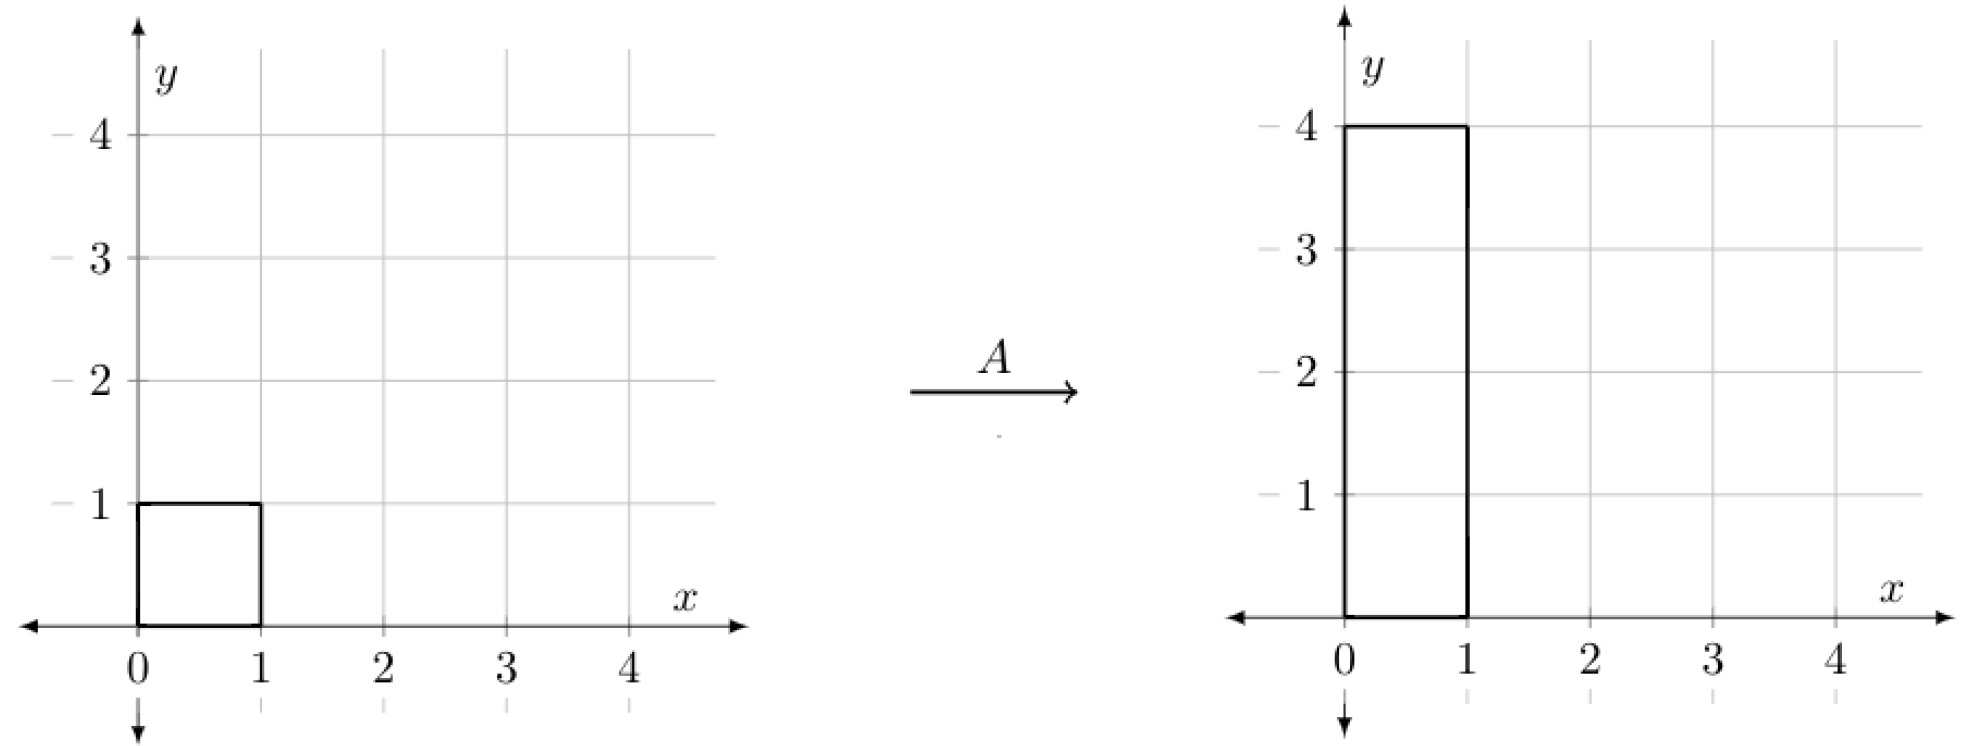
\includegraphics[scale=.6]{img/TransformationA.jpg}
\end{center}

So:  multiplication by a diagonal matrix is easy to understand.

What about $B = \mat{3&-1\\-2&2}$?  Applying this to
the same four points of the unit square $(0,0)$, $(0,1)$, $(1,0)$ and $(1,1)$
yields
$$
(0,0), (-1,2), (3,-2), (2,0)
$$
which is a completely different parallelogram, as in the figure below:

\begin{center}
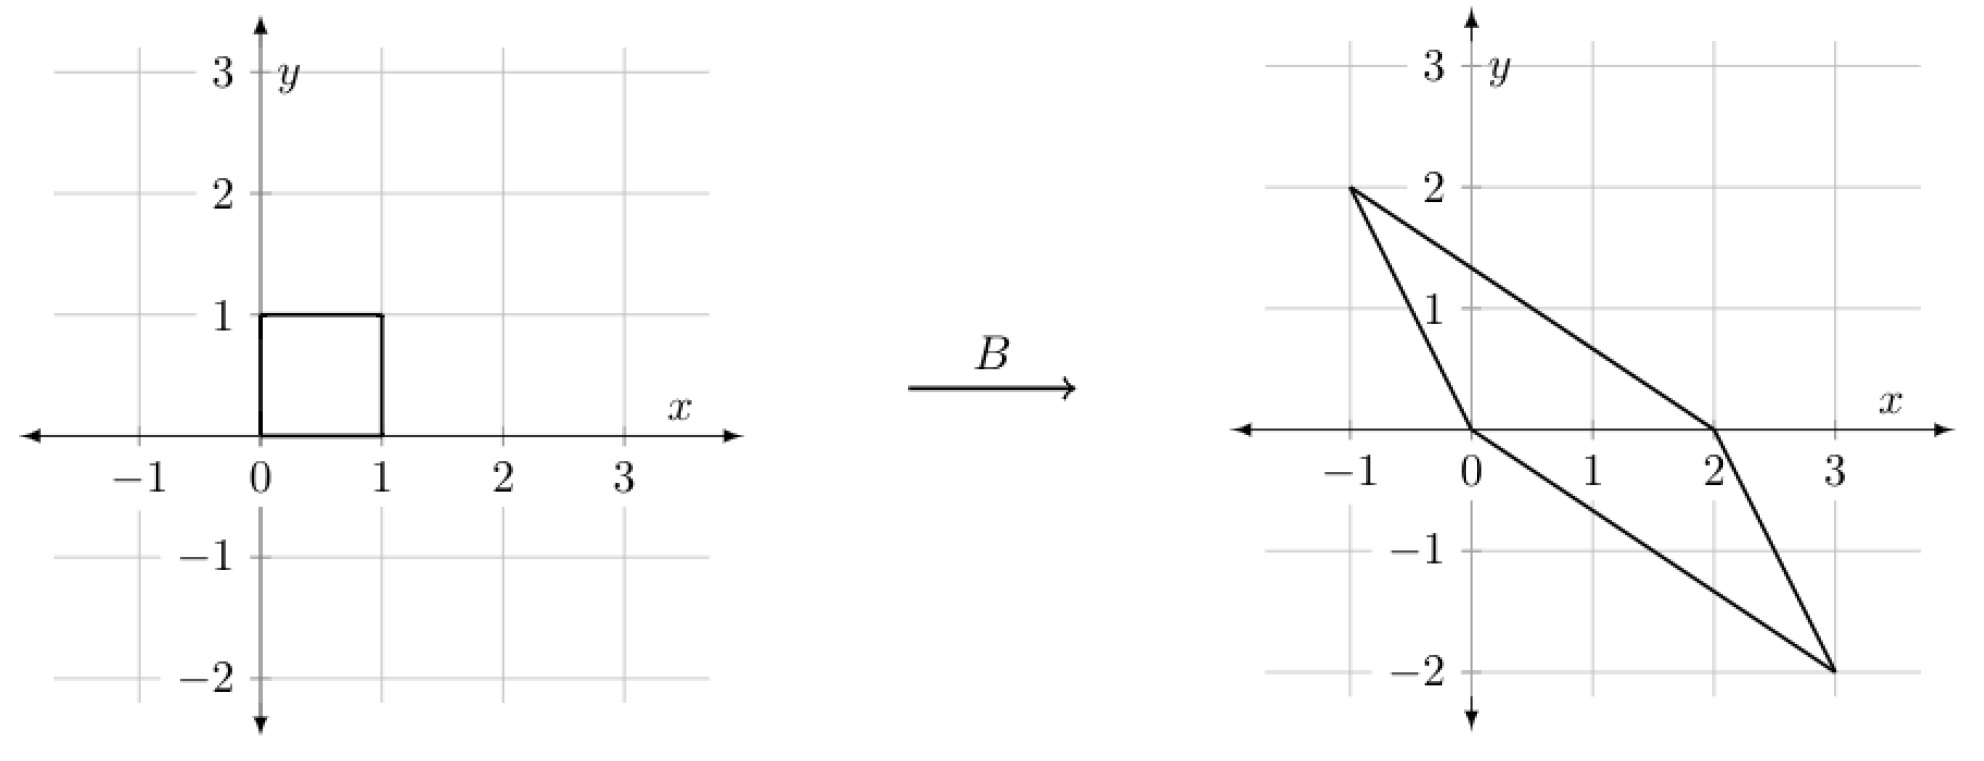
\includegraphics[scale=.6]{img/TransformationB1.jpg}
\end{center}

But what does it mean?  

The secret is in the eigenvectors.  They are $(1,2)$ (corresponding
to eigenvalue 1) and $(-1,1)$ (corresponding to eigenvalue 4).
So if we were to draw a parallelogram with vertices
$$
(0,0), (1,2), (-1,1), (0,3)
$$
then after multiplication by $B$, you'd get
$$
(0,0), (1,2), (-4,4), (-3, 6)
$$
which makes sense when you sketch it, as in the figure below:

\begin{center}
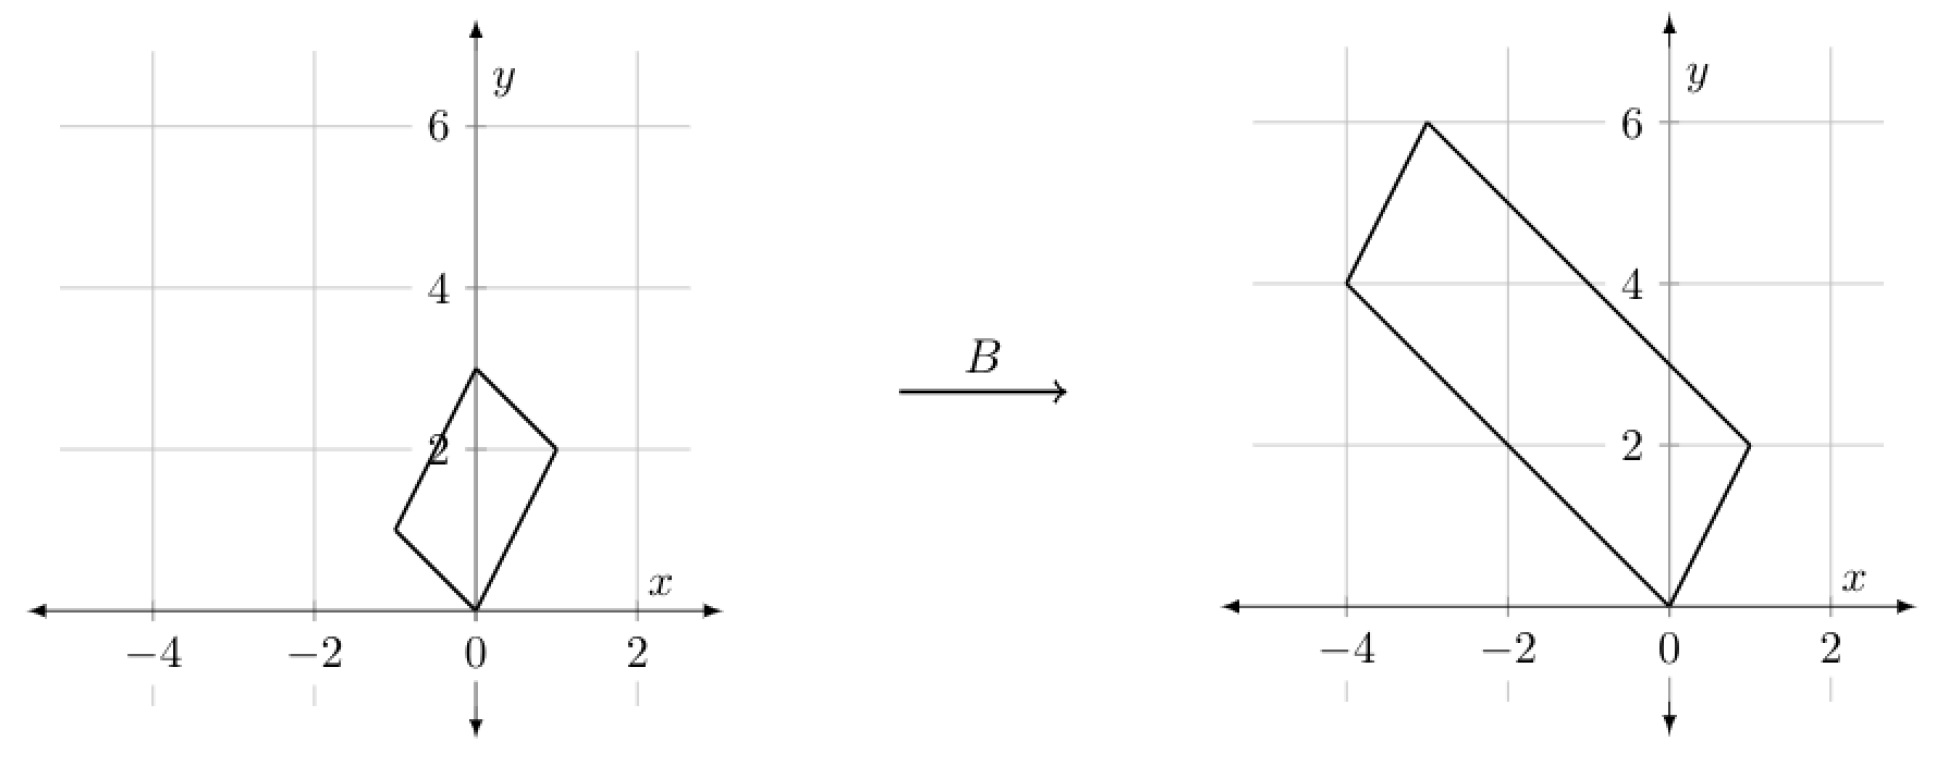
\includegraphics[scale=.6]{img/TransformationB2.jpg}
\end{center}

Multiplication by $B$ stretch the parallelogram
by a factor of $4$ in the direction $(-1,1)$ (and by a factor of $1$ in the direction $(1,2)$).
Looking back, this also explains what happened to our standard unit square:  it
was stretched along the axis $\spn\{(-1,1)\}$.

The point:  the basis of eigenvectors is the secret to understanding
the geometry of multiplication by $A$.
\end{myexample}

Viewing $A$ as a transformation in this way --- as a \stress{linear transformation} --- is fundamental to discrete time dynamical systems see  `Markov processes in probability'\footnote{Search the web for  `Markov chain'.}.


What we want to do next:  explore this idea of linear transformations in
greater detail, and get back to that picture we once used in class,
illustrating the nullspace and column space of a matrix via a map from
$\R^n$ to $\R^m$ (the map being:  multiplication by $A$).



